\section{Quality control}
\label{sec:quality}

\subsection{Flag scheme}
\label{sec:qc-flags}

Every archived record carries a composite quality flag on a three level scale.
Level 0 records satisfy every test and are used for all analyses. Level 1
records fail a test whose effect is expected to be small and are used for annual
sums but not for process studies. Level 2 records are rejected and gap filled.

\begin{table}[t]
\centering
\small
\caption{Quality control tests and the fraction of records assigned to each
level across the network in 2024. The tests are applied in the order listed and
a record takes the highest level triggered by any test.}
\label{tab:qc-tests}
\begin{tabular}{llrrr}
\toprule
Test & Criterion & Level 0 (\%) & Level 1 (\%) & Level 2 (\%) \\
\midrule
Instrument diagnostic  & analyser signal strength & 96.1 & 1.4 & 2.5 \\
Spike fraction         & fewer than 1\% removed   & 97.8 & 1.6 & 0.6 \\
Stationarity           & 30\% between subintervals & 84.2 & 9.9 & 5.9 \\
Integral turbulence    & 30\% from similarity     & 88.7 & 7.4 & 3.9 \\
Footprint              & 70\% in target class     & 93.8 & 4.1 & 2.1 \\
Friction velocity      & threshold, Section~\ref{sec:qc-ustar} & 82.6 & 0.0 & 17.4 \\
Precipitation          & no tips in interval      & 94.3 & 0.0 & 5.7 \\
\midrule
Composite              &                          & 71.9 & 19.5 & 8.6 \\
\bottomrule
\end{tabular}
\end{table}

The composite row is not the product of the individual rows because the tests are
strongly correlated: a record that fails stationarity usually also fails the
integral turbulence test, and both are concentrated in the nocturnal hours where
the friction velocity filter is already active. Data return after quality control
is the sum of the level 0 and level 1 composite fractions, 91.4 percent.

\subsection{The friction velocity threshold}
\label{sec:qc-ustar}

Under weak turbulence, the eddy covariance method underestimates the nocturnal
carbon flux because a portion of the respired carbon accumulates below the sensor
rather than passing through it. The standard remedy is to reject records below a
site specific friction velocity threshold and to gap fill them.

The threshold is determined by binning nocturnal records by friction velocity
within temperature classes and locating the point at which the binned flux
ceases to increase. Applied to the 2024 record, the thresholds range from 0.09
metres per second at the sheltered saltmarsh site MC05 to 0.15 at the exposed
dune site MC08.

\begin{figure}[t]
\centering
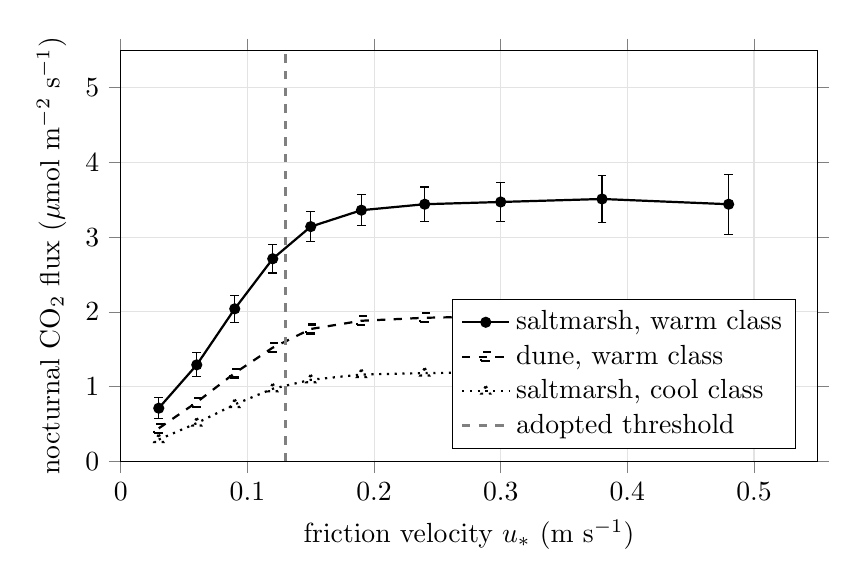
\begin{tikzpicture}
\begin{axis}[
  width=0.86\textwidth, height=6.8cm,
  xlabel={friction velocity $u_*$ (m s$^{-1}$)},
  ylabel={nocturnal CO$_2$ flux ($\mu$mol m$^{-2}$ s$^{-1}$)},
  xmin=0, xmax=0.55, ymin=0, ymax=5.5,
  legend pos=south east, legend cell align=left,
  grid=both, grid style={gray!22}, tick align=outside
]
\addplot[thick,mark=*,mark size=1.6pt,error bars/.cd,y dir=both,y explicit]
 coordinates {
  (0.03,0.71) +- (0,0.14) (0.06,1.29) +- (0,0.16) (0.09,2.04) +- (0,0.18)
  (0.12,2.71) +- (0,0.19) (0.15,3.14) +- (0,0.20) (0.19,3.36) +- (0,0.21)
  (0.24,3.44) +- (0,0.23) (0.30,3.47) +- (0,0.26) (0.38,3.51) +- (0,0.31)
  (0.48,3.44) +- (0,0.40)
};
\addlegendentry{saltmarsh, warm class}
\addplot[thick,dashed,mark=square,mark size=1.6pt] coordinates {
  (0.03,0.44) (0.06,0.79) (0.09,1.18) (0.12,1.52) (0.15,1.77)
  (0.19,1.88) (0.24,1.92) (0.30,1.94) (0.38,1.95) (0.48,1.93)
};
\addlegendentry{dune, warm class}
\addplot[thick,dotted,mark=triangle,mark size=1.8pt] coordinates {
  (0.03,0.29) (0.06,0.51) (0.09,0.76) (0.12,0.97) (0.15,1.09)
  (0.19,1.16) (0.24,1.18) (0.30,1.19) (0.38,1.20) (0.48,1.18)
};
\addlegendentry{saltmarsh, cool class}
\addplot[gray,thick,dashed] coordinates {(0.13,0) (0.13,5.5)};
\addlegendentry{adopted threshold}
\end{axis}
\end{tikzpicture}
\caption{Binned nocturnal carbon flux against friction velocity for two land
cover classes and two temperature classes. Each curve reaches a plateau, and the
threshold is placed where the binned flux first exceeds 99 percent of the
plateau value. Error bars are the standard error of the bin mean and are shown
for one curve only.}
\label{fig:ustar-threshold}
\end{figure}

Figure~\ref{fig:ustar-threshold} shows the underlying relationship. The plateau
is well defined in the warm classes and less so in the cool classes, where the
flux is small and the bin standard error is a larger fraction of it. The
network wide threshold of 0.13 metres per second, shown as the vertical line, is
used for the headline budget, and the sensitivity to that choice is quantified
in Section~\ref{sec:results-uncertainty}.

\subsection{Energy balance closure}
\label{sec:qc-closure}

Energy balance closure is the standard independent check on a flux measurement.
Over the year the network closes to $0.84 \pm 0.03$, meaning that the sum of the
turbulent fluxes accounts for 84 percent of the available energy. This is within
the range reported for coastal sites and is not evidence of a specific error,
but the residual is not random: it is largest at midday and largest at the dune
sites, which is the signature of an unmeasured advective term rather than of
instrument bias \citep{ridley2019closure}.

The radiometer drift of Section~\ref{sec:instr-slow} accounts for approximately
3 percentage points of the closure deficit. Reprocessing against the returned
calibration coefficients improved the annual closure from 0.81 to 0.84.
